\documentclass[a4paper,11pt]{article}
\usepackage[a4paper, margin=1.8cm]{geometry}
% Encodage de caractère
\usepackage[T1]{fontenc} 
% Définit l'encodage UTF-8
\usepackage[utf8]{inputenc}
% Permet la gestion des particularités linguistiques 
% propres à la langue française
\usepackage[french]{babel}
% Pour la gestion de couleurs
\usepackage{xcolor}
% Permet la personalisation de la table de matières
\usepackage{tocloft} 
% sert à personnaliser les listes
\usepackage{enumitem} 
% Pour gérer les liens hypertextes et urls
\usepackage{hyperref} 
% Pour les fonctionnalités mathématiques
\usepackage{amsmath} 
% Ajoute les polices mathématiques
\usepackage{amsfonts} 
% Gère les images
\usepackage{graphicx} 
 % Pour gérer les citations et les guillemets
\usepackage[style=english]{csquotes}
% Permet la gestion de tableaux extensibles
\usepackage{tabularx} 
% Pour fusionner les cellules sur plusieurs lignes dans un tableau
\usepackage{multirow} 

\usepackage{upquote}

\usepackage{tcolorbox}

\usepackage{verbatim}

\usepackage{longtable}

\usepackage{listings}


% Indique le titre du document
\title{Pogrammation Impérative}
\author{PULUDISU \bsc{Mpia Mimpiya}\\Numéro étudiant: 18913467 \\ L1 Informatique}
\date{\today}

% Personalisation de la table de matières
% change la couleur de texte de sections et sous-sections en bleu et 
% met les sections en gras
\renewcommand{\cftsecfont}{\color{blue}\normalfont}
\renewcommand{\cftsubsecfont}{\color{blue}\normalfont}
\renewcommand{\cftsecfont}{\bfseries}

% définit la couleur urls et liens hypertextes en bleu
\hypersetup{colorlinks=true,linkcolor=blue,urlcolor=blue}

\lstset{
    language=C,
    basicstyle=\ttfamily\small,
    keywordstyle=\color{blue}\bfseries,
    commentstyle=\color{gray},
    stringstyle=\color{red},
    numbers=none,
    numberstyle=\tiny\color{gray},
    stepnumber=1,
    numbersep=10pt,
    backgroundcolor=\color{gray!2},
    tabsize=4,
    captionpos=b,
    breaklines=true,
    breakatwhitespace=false,
    showspaces=false,
    showstringspaces=false,
    showtabs=false,
    frame=single,
    framesep=10pt,
    framerule=0.1pt,
    aboveskip=10pt,
    belowskip=10pt,
    inputencoding=utf8,
    extendedchars=true,
    xleftmargin=0pt, % Ajustez cette valeur pour le padding à gauche
    xrightmargin=5mm,
    literate=%
        {é}{{\'e}}1
        {è}{{\`e}}1
        {à}{{\`a}}1
        {ç}{{\c{c}}}1
        {ê}{{\^e}}1
        {ë}{{\"e}}1
        {â}{{\^a}}1
        {î}{{\^i}}1
        {ï}{{\"i}}1
}

\tcbuselibrary{listingsutf8}

\begin{document}
   %
  \maketitle
  %

  % Table de matières
  \tableofcontents

  % Force le contenu qui suit à se mettre dans une nouvelle page
    \newpage
    \section{Attendus}
      \noindent Pour ce cours, nous devons rendre 
      les exercices cx17.4, cx17.7 et cx17.8 de la série cx17 et les exercices  cx25.0 et cx25.1 de la série cx25.
      Comme certains exercices dépendent d'autres exercices dans le cours, j'ai ajouté exercice cx15.3 de la série cx15 et les exercices cx18.1 et cx18.6 
      de la série cx18. 
       
    \newpage
    \section{Série cx18}
      \subsection{cx18.1: Recoder la fonction putlist() pour afficher la liste en ordre inverse}
        \noindent
        \lstinputlisting{codes/cx18/cx18.1/data.c}

        \noindent Dans le programme ci-dessus, recoder la fonction putlist() pour qu'elle affiche la liste en
        ordre inverse, i.e. l'ordre dans lequel les éléments ont été rencontrés et empilés.
        
        \bigskip
        \noindent Pour afficher la liste en ordre inverse, nous devons inverser la liste avant de l'afficher, 
        voici un petit programme qui réalise cette tâche: 

        \lstinputlisting{codes/cx18/cx18.1/cx18.1.c}

        \bigskip
        \noindent Nous pouvons compiler et lancer le programme: 
        \begin{tcolorbox}[colback=lightgray!6, colframe=black, left=-20mm, right=5mm, top=2mm, bottom=-2mm, boxrule=0.1mm]
          \begin{verbatim}
            gcc -W cx18.1.c -o cx18.1
            ./cx18.1
          \end{verbatim}
        \end{tcolorbox}
    
        \subsection{cx18.6: Déporter les fonctions de gestion de listes dans une bibliothèque dynamique}

        \noindent Adapter votre solution de [cx18.1] en déportant les fonctions de gestion de listes dans une
        bibliothèque dynamique – vérifier que le programme tourne toujours. \\
        Essayer d'adapter de la même façon les autres exemples de la série...

        \bigskip
        \noindent Pour déporter les fonctions de gestion de listes dans une bibliothèque dynamique, 
        nous allons créer les fichiers suivants dans la même arborecence: 
        \begin{enumerate}
          \item \texttt{list.h}: pour les déclarations. Voici le code de ce fichier: 
            \lstinputlisting{codes/cx18/cx18.6/list.h}
          \newpage
          \item \texttt{list.c}: pour les définitions. Voici le code de ce fichier:
            \lstinputlisting{codes/cx18/cx18.6/list.c}
          \item Et \texttt{main.c}: pour le programme principal. Voici le code de ce fichier:
            \lstinputlisting{codes/cx18/cx18.6/main.c}
        \end{enumerate}
        \noindent Pour compiler et exécuter le programme,voici les étapes à suivres :

        \begin{enumerate}
          \item Compilation et création de la bibliothèque dynamique:
            \begin{itemize}
              \item Compilez le fichier \texttt{list.c} pour créer un objet partagé :
                \begin{tcolorbox}[colback=lightgray!6, colframe=black, left=-20mm, right=5mm, top=2mm, bottom=-2mm, boxrule=0.1mm]
                  \begin{verbatim}
                    gcc -c -fPIC list.c -o list.o
                  \end{verbatim}
                \end{tcolorbox}
              \item Créez la bibliothèque dynamique à partir de l'objet partagé :
                \begin{tcolorbox}[colback=lightgray!6, colframe=black, left=-20mm, right=5mm, top=2mm, bottom=-2mm, boxrule=0.1mm]
                  \begin{verbatim}
                    gcc -shared -o liblist.so list.o
                  \end{verbatim}
                \end{tcolorbox}
              \item Compilez le programme principal en liant la bibliothèque dynamique :
                \begin{tcolorbox}[colback=lightgray!6, colframe=black, left=-20mm, right=5mm, top=2mm, bottom=-2mm, boxrule=0.1mm]
                  \begin{verbatim}
                    gcc -o main main.c -L. -llist
                  \end{verbatim}
                \end{tcolorbox}
            \end{itemize}
          \item Exécuter le programme: Pour exécuter le programme, nous devons nous assurer que le système peut trouver la bibliothèque dynamique. 
          Nous définissons la variable d'environnement \texttt{LD\_LIBRARY\_PATH} pour inclure le répertoire courant :

          \begin{tcolorbox}[colback=lightgray!6, colframe=black, left=-20mm, right=5mm, top=2mm, bottom=-2mm, boxrule=0.1mm]
            \begin{verbatim}
              export LD_LIBRARY_PATH=.:$LD_LIBRARY_PATH
              ./main
            \end{verbatim}
          \end{tcolorbox}
        \end{enumerate}

        \bigskip
        \noindent Si toutes les étapes sont respectées, on devait avoir \texttt{h g f e d c b a}.
        
    \newpage
    \section{Série cx15}
      \subsection{cx15.3: Créer le fichier texte \texttt{cx15.3.data} et lire les données dans une table de chaînes}
        \noindent Voici le contenu du fichier \texttt{cx15.3.data}:
        \lstinputlisting{codes/cx15/cx15.3/cx15.3.data}

        \bigskip
        \noindent notre petit programme: 
        \lstinputlisting{codes/cx15/cx15.3/main.c}

        \noindent La compilation et l'exécution du programme:
        \begin{tcolorbox}[colback=lightgray!6, colframe=black, left=-20mm, right=5mm, top=2mm, bottom=-2mm, boxrule=0.1mm]
          \begin{verbatim}
            gcc -W main.c -o main
            ./main
          \end{verbatim}
        \end{tcolorbox}

        \noindent La sortie du programme est: 
        \begin{tcolorbox}[colback=lightgray!6, colframe=black, left=-20mm, right=5mm, top=2mm, bottom=-2mm, boxrule=0.1mm]
          \begin{verbatim}
            Joe
            Jack
            William
            Averell
          \end{verbatim}
        \end{tcolorbox}
        
      
    \newpage
    \section{Série cx17}
        \subsection{cx17.2: Utiliser la solution de [cx15.3] pour lire et exploiter une STOPLIST}
          \noindent Utiliser votre solution de [cx15.3] pour rajouter au programme la capacité de lire et d'exploiter
          une STOPLIST comme dans le prototype PYTHON.

          \bigskip
          \noindent Pour cette étape, nous allons lire une STOPLIST à partir d'un fichier et l'utiliser pour filtrer 
          les mots lus dans cx15.3.data.

          \bigskip
          \noindent Voici les fichiers de notre arborecence:
          
          \begin{figure}[ht]
            \makebox[\textwidth][l]{
                \hspace{0.4cm}
                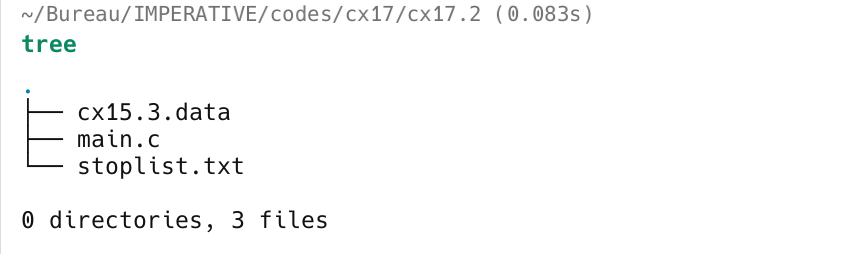
\includegraphics[width=0.6\textwidth]{codes/cx17/cx17.2/tree.png}
            }
          \end{figure}

        \noindent Voici le programme principal:
        \lstinputlisting{codes/cx17/cx17.2/main.c}

        \noindent La compilation et l'exécution du programme:
        \begin{tcolorbox}[colback=lightgray!6, colframe=black, left=-20mm, right=5mm, top=2mm, bottom=-2mm, boxrule=0.1mm]
          \begin{verbatim}
            gcc -W main.c -o main
            ./main
          \end{verbatim}
        \end{tcolorbox}

        \noindent La sortie du programme est: 
        \begin{tcolorbox}[colback=lightgray!6, colframe=black, left=-20mm, right=5mm, top=2mm, bottom=-2mm, boxrule=0.1mm]
          \begin{verbatim}
            William
            Averell
          \end{verbatim}
        \end{tcolorbox}
      
      \newpage
      \subsection{cx17.6: Utiliser une STOPLIST représentée en interne sous la forme d'une liste élastique}

        \noindent Utiliser votre solution de [cx15.3] et de [cx17.2] pour ajouter au programme la capacité
        d'accueillir et d'exploiter une STOPLIST représentée en interne sous la forme d"une liste
        élastique, et lue à partir d'un fichier dont le nom sera spécifié sur la LdC — s'il ne l'est pas,
        le programme ouvrira un fichier par défaut.
        
        \bigskip
        \noindent Pour cet exercice, nous allons utiliser une liste chaînée pour représenter la STOPLIST.

        \bigskip
        \noindent Pour réaliser cet exercice, voici les fichiers de notre arborecence:
        
        \begin{figure}[ht]
          \makebox[\textwidth][l]{
              \hspace{0.4cm}
              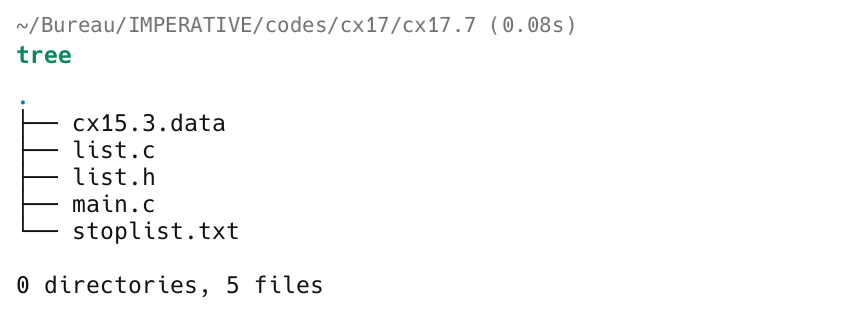
\includegraphics[width=0.6\textwidth]{codes/cx17/cx17.6/tree.png}
          }
        \end{figure}

        \noindent Nous allons nous attarder sur les trois fichiers principaux:
        \begin{enumerate}
          \item \texttt{list.h}:
            \lstinputlisting{codes/cx17/cx17.6/list.h}
          \item \texttt{list.c}:
            \lstinputlisting{codes/cx17/cx17.6/list.c}
          \item \texttt{main.c}:
            \lstinputlisting{codes/cx17/cx17.6/main.c}
        \end{enumerate}

        \noindent La compilation et l'exécution du programme:
        \begin{tcolorbox}[colback=lightgray!6, colframe=black, left=-20mm, right=5mm, top=2mm, bottom=-2mm, boxrule=0.1mm]
          \begin{verbatim}
            gcc -c list.c -o list.o
            gcc -c main.c -o main.o
            gcc main.o list.o -o main
            ./main
          \end{verbatim}
        \end{tcolorbox}

        \bigskip
        \noindent La sortie du programme, on a le résultat suivant en prenant compte de notre \texttt{cx15.3.data} et de notre \texttt{stoplist.txt}:
        \begin{tcolorbox}[colback=lightgray!6, colframe=black, left=-20mm, right=5mm, top=2mm, bottom=-2mm, boxrule=0.1mm]
          \begin{verbatim}
            William
            Averell
          \end{verbatim}
        \end{tcolorbox}

      \newpage
      \subsection{cx17.7: Adapter la solution de [cx17.6] pour utiliser la bibliothèque créée pour [cx18.6]}
        \noindent Adapter votre solution de [cx17.6] pour utiliser la bibliothèque créée pour [cx18.6].

        \bigskip
        \noindent Pour cette étape, nous allons utiliser la bibliothèque créée pour [cx18.6].

        \bigskip
        \noindent Cet exercice est presque similaire à [cx17.6], nous allons donc aller rapidement:

        \bigskip
        \noindent Voici les codes de fichiers principaux:

        \begin{enumerate}
          \item \texttt{list.h}:
            \lstinputlisting{codes/cx17/cx17.7/list.h}
          \item \texttt{list.c}:
            \lstinputlisting{codes/cx17/cx17.7/list.c}
          \item \texttt{main.c}:
            \lstinputlisting{codes/cx17/cx17.7/main.c}
        \end{enumerate}

        \noindent
        \noindent La compilation et l'exécution du programme, voici les étapes à suivre:
        \begin{enumerate}
          \item \textbf{Compilation et création de la bibliothèque dynamique}
            \begin{enumerate}
              \item Compilez le fichier \texttt{list.c} pour créer un objet partagé :
                \begin{tcolorbox}[colback=lightgray!6, colframe=black, left=-20mm, right=5mm, top=2mm, bottom=-2mm, boxrule=0.1mm]
                  \begin{verbatim}
                    gcc -c -fPIC list.c -o list.o
                  \end{verbatim}
                \end{tcolorbox}
              \item Créez la bibliothèque dynamique à partir de l'objet partagé :
                \begin{tcolorbox}[colback=lightgray!6, colframe=black, left=-20mm, right=5mm, top=2mm, bottom=-2mm, boxrule=0.1mm]
                  \begin{verbatim}
                    gcc -shared -o list.so list.o
                  \end{verbatim}
                \end{tcolorbox}
              \item Compilez le programme principal en liant la bibliothèque dynamique :
                \begin{tcolorbox}[colback=lightgray!6, colframe=black, left=-20mm, right=5mm, top=2mm, bottom=-2mm, boxrule=0.1mm]
                  \begin{verbatim}
                    gcc -o main main.c -L. -llist
                  \end{verbatim}
                \end{tcolorbox}
            \end{enumerate}
          \item \textbf{Exécution du programme}
            \begin{tcolorbox}[colback=lightgray!6, colframe=black, left=-20mm, right=5mm, top=2mm, bottom=-2mm, boxrule=0.1mm]
              \begin{verbatim}
                export LD_LIBRARY_PATH=.:$LD_LIBRARY_PATH
                ./main
              \end{verbatim}
            \end{tcolorbox}
        \end{enumerate}

      \subsection{cx17.8: Adapter la solution de [cx17.6] pour utiliser la bibliothèque créée pour [cx18.7]}

        \begin{enumerate}
          \item \texttt{list.h}:
            \lstinputlisting{codes/cx17/cx17.8/list.h}
          \item \texttt{list.c}:
            \lstinputlisting{codes/cx17/cx17.8/list.c}
          \item \texttt{main.c}:
            \lstinputlisting{codes/cx17/cx17.8/main.c}
        \end{enumerate}

        \bigskip
        \noindent Pour compiler et exécuter le programme, voir l'exercice cx17.7 c'est quasi le même processus.

    \newpage
    \section{Série cx25}

      \subsection{cx25.0: Programmer cet émulateur de sorte qu'il puisse lire le code numérique (ou symbolique) à partir d'un fichier}

        \bigskip
        \noindent Ce petit programme écrit en C simule un processeur simple avec une mémoire de taille fixe et un ensemble d'instructions de base. 
        Il charge un programme à partir d'un fichier (program.hex), l'exécute et affiche l'état de l'accumulateur (A) et du compteur de programme (PC) 
        à chaque étape.

        \lstinputlisting{codes/cx25/cx25.0/cx25.0.c}

        \bigskip
        \noindent Pour compiler et exécuter le programme, merci de faire:
        \begin{tcolorbox}[colback=lightgray!6, colframe=black, left=-20mm, right=5mm, top=2mm, bottom=-2mm, boxrule=0.1mm]
          \begin{verbatim}
            gcc -W cx25.0.c -o main
            ./main program.hex
          \end{verbatim}
        \end{tcolorbox}

        \begin{figure}[ht]
          \makebox[\textwidth][l]{
              \hspace{0.3cm}
              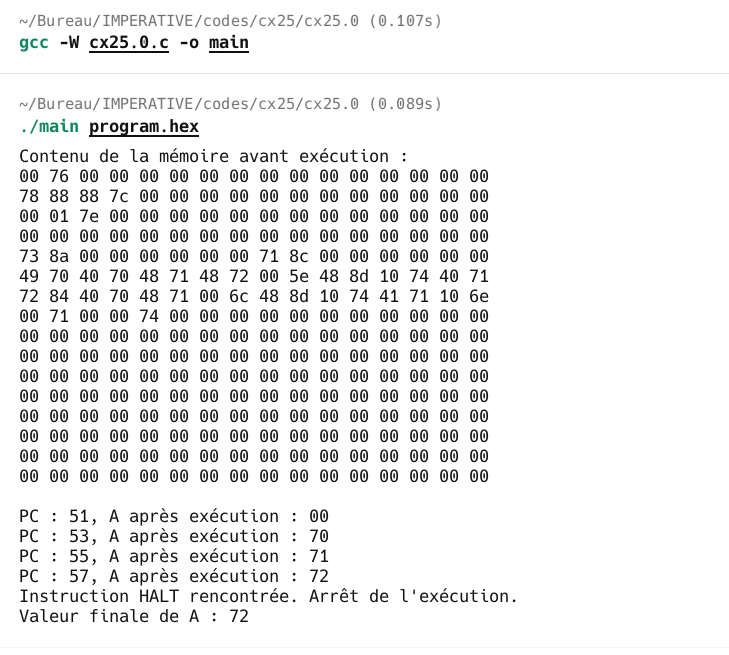
\includegraphics[width=\textwidth]{codes/cx25/cx25.0/screen.png}
          }
        \end{figure}

      \newpage
      \subsection{cx25.1: Coder la boucle d'évaluation pour en faire un STEPPER}
        \noindent Coder la boucle d'évaluation pour en faire un STEPPER qui affiche la valeur de PC et de A, et
        attend confirmation au clavier pour exécuter l'instruction suivante!; développez-le pour
        émuler celles des fonctionnalités de gdb qui vous paraissent utiles — ou faciles.

        \bigskip
        \noindent Ce petit programme écrit en C simule un processeur simple avec une mémoire de taille fixe et un ensemble d'instructions de base. 
        Il charge un programme à partir d'un fichier (program.hex), l'exécute et affiche l'état de l'accumulateur (A) et du compteur de programme (PC) 
        à chaque étape. A la différence de cx25.0, le programme attend confirmation au clavier pour exécuter l'instruction suivante.

        \newpage
        \noindent Voici le code source:
        
        \lstinputlisting{codes/cx25/cx25.1/cx25.1.c}

        \bigskip
        \noindent Il ne reste plus qu'à compiler et exécuter notre programme:

        \begin{tcolorbox}[colback=lightgray!6, colframe=black, left=-20mm, right=5mm, top=2mm, bottom=-2mm, boxrule=0.1mm]
          \begin{verbatim}
            gcc -W cx25.1.c -o main
            ./main program.hex 
          \end{verbatim}
        \end{tcolorbox}

        \begin{figure}[ht]
          \makebox[\textwidth][l]{
              \hspace{0.4cm}
              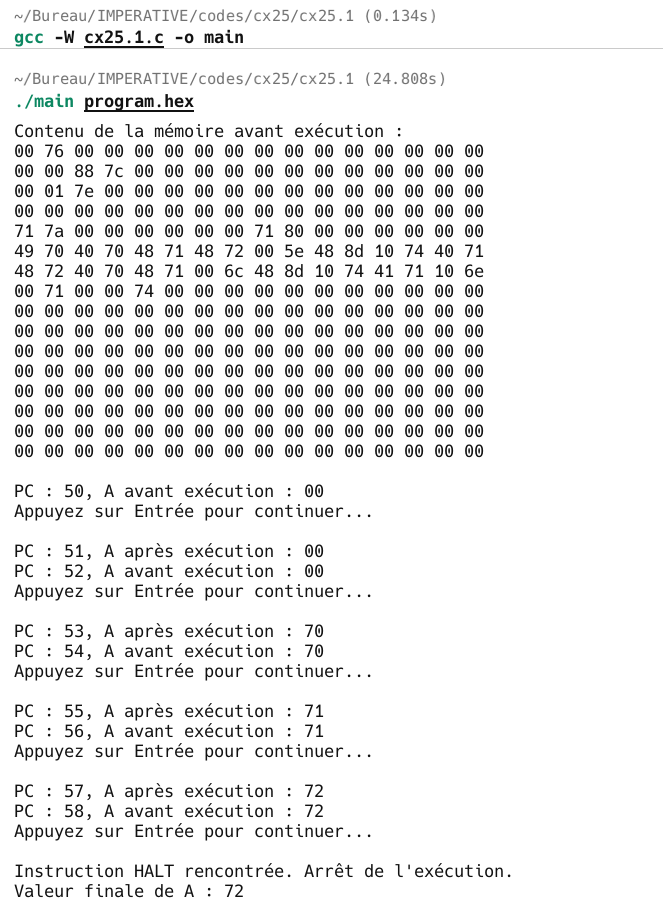
\includegraphics[width=0.8\textwidth]{codes/cx25/cx25.1/screen.png}
          }
        \end{figure} 
\end{document}